\documentclass[../report.tex]{subfiles}
\begin{document}

\section {数据库设计}

\subsection {数据库设计需求}

学校有多个校区,各个校区均有其校区代码(唯一)、校区名称和校区地址
(实体中包括但不限于上述属性,下同)。学校开设多个专业,各个专业均有其
专业代码(唯一)、专业名称、专业地址、专业负责人和所属校区(一个专业仅
属于一个校区)。学校建立多个班级,各个班级均有其班级代码(唯一)、班级
名称、建班年月、班主任、所属年级(年份)和所属专业。

学校将所有教师和学生的基本个人信息统一存放,包括身份证件号(唯一)、
身份证件类型(身份证或护照)、中文名称、性别码(女或男)、出生日期(年
月日)和国籍(中文名称)。如果教师和学生提供了家庭通讯方式,包括家庭住
址、家庭邮政编码和家庭电话,学校也会记录。每个教师也有属于自己的工号(唯
一),每个学生有属于自己的学号(唯一)。学校记录学生的入学年月、电子邮
箱和所属班级,也记录教师的入职年月、电子邮箱、所属专业和职称(教授或副
教授)。学校允许学生转专业和降级(二者不同时发生,转专业和降级时均转班,
且只允许一次转专业和一次降级),统称为学籍异动。学生发生学籍异动时需要
记录异动编号(唯一,同一学生转专业和降级各有不同的异动编号)、异动日期
(年月)、原班级代码和现班级代码。转专业还需要记录是否已转出团员关系(是、
否或不是团员),降级则还需要记录降级原因(休学或支教)。

学校开设不同课程,每门课程均有其课程号(唯一,与课程名称一一对应)、
课程名称、开课专业和考核方式(考试或当堂答辩,满分均为 100)。当一门课
程开课时,需要记录其授课教师(一门课仅有一个授课教师)、开课日期(年)、
开课学期(春或秋)、开课时间(每个课程一周只开一节课,为周一至周五的第
一节至第九节中的某一节,自定义记录方式)。学校会记录每个学生的选课记录
(不允许重复选课),包括选课日期(同开课日期)、选课学期(同开课学期)
和考试成绩。

\subsection {数据库设计与改良}

这里结合第二次实验的设计报告,去给出我们最初选择的数据库设计。

\begin{figure}[H]
\centering
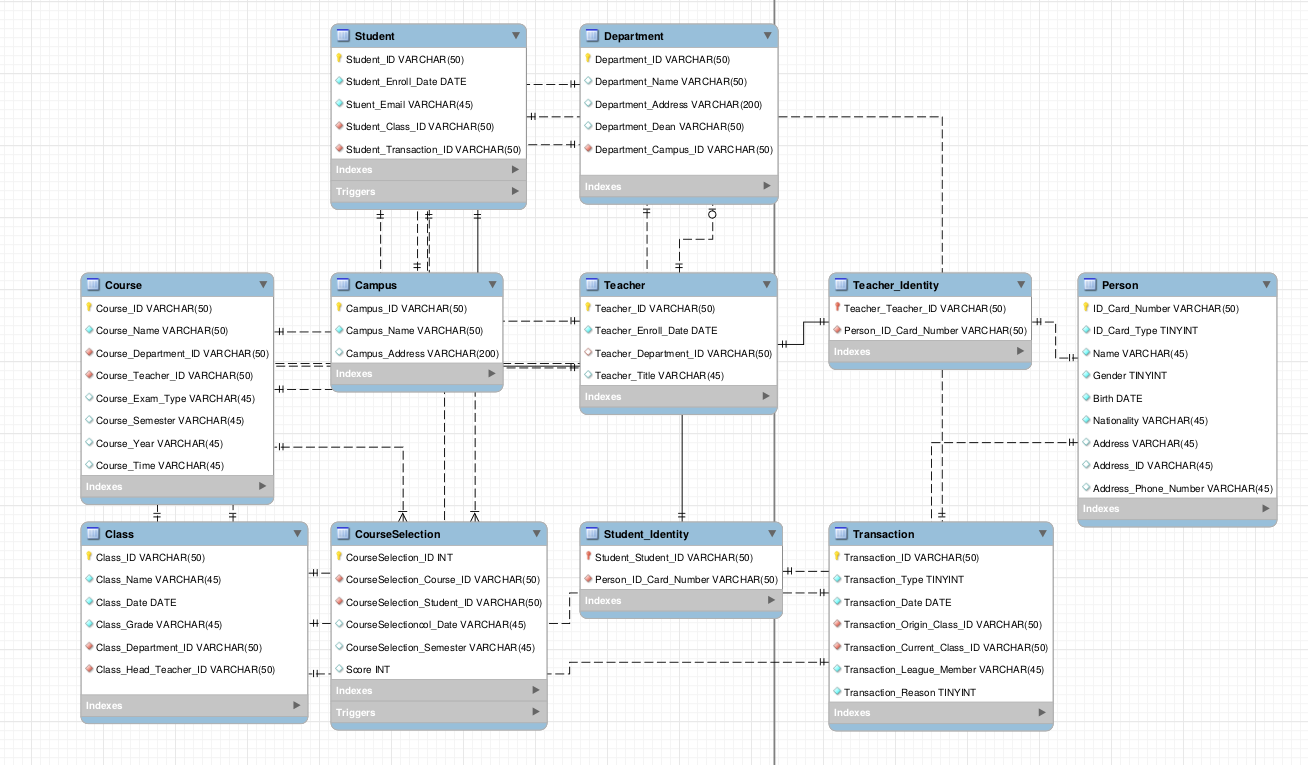
\includegraphics[width=1\linewidth]{../figure/database-design.png}
\caption{数据库设计一览}
\label{fig:database-design}
\end{figure}

在实际实现的时候,大家迅速发现了问题,单独列出Student\_Identity表,对于我们的信息维护几位不方便。所以最终,在这一版数据库的基础上,我们给Student和Teacher分别增加了一个外健,用于和Person链接。

最终用于生成数据库框架的代码:
\MYhref{https://github.com/KradNosnatef/996_SQL/blob/master/src/main/resources/sql_init.sql}{\underline{database-init-github-link}}

\section{管理系统总体框架的设计}

我们的框架基本按照一般的前后端分离的办法操作。

Login Servlet 是我们应用的大门,用于处理登陆信息。

User-Type 是我们登陆后第一个需要审查的元素。 我们通过他来判断我们的用户的类别。

我们的用户分为3个基本类别:

1. \texttt{Admin Account} 有所有功能的权限

2. \texttt{Student Account} 只有部分查询权限,可以对自己的个人信息修改

3. \texttt{Teacher Account} 只有煮粉查询权限,可以查询所有学生信息,可以对自己的个人信息修改

\begin{figure}[H]
\centering
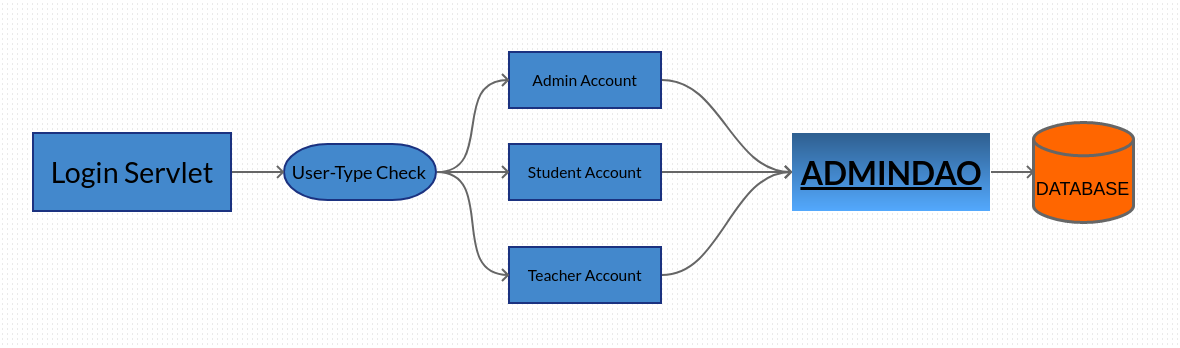
\includegraphics[width=1.1\linewidth]{figure/framework}
\caption{framework}
\label{fig:untitledpage}
\end{figure}

我们管理权限主要是利用前端强制管理,这里是我们设计的不足之处。在对应的用户页面上之开放他能用的功能。但是,如果用户足够细心和好运,他可以通过观察我们发出的HTTP Request从而对我们的信息进行解析。继而通过Postman等工具,发送请求,就可以轻松获取自己权限以外的操作。

正确的做法是,处理所有HTTP请求是,处理带上session或者token,记录下用户的类型。此外,对于java servlet发送的请求,我们应当适度做一些加密操作。

\section{后端设计}

\subsection{一览}

后端大体框架为4部分:
\begin{itemize}
\itemsep -0.3em
\ttfamily
\item DAO: Data Access Object 主要用来做各种实体的数据库操作 
\item model: 存放各种实体的数据类型
\item service: 存放各种 Java Serrvlet 服务
\item utils: 常用API的单独存放
\end{itemize}

\subsection{utils}

这里我没有按照字典序介绍,而是理解由易到难的次序介绍。

首先是utils里的各个模块:

\begin{enumerate}
\itemsep 0em
\ttfamily 
\item Datautils 处理我们 Data 等特殊格式的数据的格式标准化
\item DButils 处理我们的数据库连接和断开的操作
\item UnitTestSwitch 用于切换本地 JDBC 数据库和 Tomcat 的 JDBI 数据库连接方式,这一模块只存放一个常量,可以理解成 Java 下的条件编译,目的是为了方便的单元测试
\end{enumerate}

\subsection{model}

对各个基本实体做存储,为各个实体做了一层封装。

\begin{enumerate}
\itemsep 0em
\ttfamily 
\item Campus 存储校区信息
\item Class 存储班级信息
\item Course 存储课程信息
\item Department 存储专业信息
\item Person 存储个人基本信息
\item Student 存储学生特有信息
\item Teacher 存储教师特有信息
\item Transaction 存储异动信息
\item Users 存储用户信息,用于系统登陆
\end{enumerate}

类型细节见程序注释。

\subsection{DAO}

这一部分为程序的核心,用于处理我们的数据库操作。我们的数据库和Java程序全是依靠他们进行连接。

我们这里不论我们的DAO母体,我们有一些公共的设计规则:
\begin{enumerate}
\ttfamily
\item 插入方法的规则\\
名称:\\
insert[Model\_Name]\\
输入:\\
对于所有的插入方法,参数为我们建立Dao对应母体的Class Model的所有需要的参数。\\
输出:\\
如果插入成功,返回非0数值,为SQL DML(Data Manipulation Language)的行号。\\
如果插入失败,返回0。如果插入成功,返回非0数值,为SQL DML(Data Manipulation Language)的行号。\\
如果插入失败,返回0。
\item 删除方法的规则\\
名称:\\
delete[Model\_Name]\\
输出:\\
对于所有的删除方法,参数为(String element\_selector, int type)\\
element\_selector 为我们的选择子,用于选定我们待删除的对象。\\
type 用于选择我们的选择子的含义。\\
我们只提供了“合理”的删除方法。这里的合理定义是符合一般常理的,例如根据院长去删除一个专业,这种事情听起来即不合理,且极容易发生操作失误。这类借口我们一律不予提供。\\
输出:\\
如果返回值为0, 待删除元素不存在。\\
如果返回值为1, 删除成功。\\
如果返回值为-1, 数据库操作异常。
\item 查询方法的规则
名称:\\
query[Model\_Name]\\
输入:\\
对于所有的查询方法,参数为(String element\_selector, int type)\\
element\_selector 为我们的选择子,用于选定我们待查询的对象。\\
type 用于选择我们的选择子的含义。\\
type = -1 表示查询所有元素的所有信息。\\
输出:\\
一个ArrayList<Model>,Model为DAO对应母体的类型。
\item 更新方法的规则
名称:\\
update[Model\_Name]\\
对于所有的更新方法,我们有两种类型:
\begin{itemize}
\item 
Update Detail Mode\\
输入:\\
参数为(int old\_type, int new\_type, String old\_value, String new\_value)\\
old\_XXX用于确定我们的更改目标,old\_type用于说明old\_value的含义。old\_value则是我们的目标的选择子。\\
new\_type指定说明我们的目标更改项,目标项的new\_type代表的属性,需要更新为new\_value。\\
输出:\\
整数,1,代表成功;0,代表失败。
\item 
Rebuild Update Mode\\
输入:\\
这里需要输入了一个基本的用于定位元素的键值,一般是主键,当然,特定情况也有其他的选择方案。其余的输入则是我们希望或者说允许更新的元素。\\
简而言之,我们这里所说的更新和插入基本是一样的。所以称为Rebuild Update Mode。
\end{itemize}

\end{enumerate}

下面我将用代码注释说明各个方法的作用。

\subsubsection{CampusDao}
用于对校区进行数据库操作。
\begin{enumerate}
\ttfamily 
\item 插入校区\\
insertCampus(String id, String name, String address)
\begin{lstlisting}[language=java, backgroundcolor=\color{lightgray}]
    // Insert new campus element
    // Input:
    // - id: campus id
    // - name: campus name
    // - address: campus address
    // Ouput:
    // - If insertion action succeed, return a number, which stands for the row count for SQL Data Manipulation
    // Language (DML) statements. Otherwise, it will return 0
\end{lstlisting}

\item 删除校区\\
deleteCampus(String element\_selector, int type)
\begin{lstlisting}[language=java, backgroundcolor=\color{lightgray}]
    // Delete a campus
    // Input:
    // - element_selector: a string used to select element
    // - type: type is used to select the meaning of element_selector
    //   type = 0 -- delete by id
    //   type = 1 -- delete by name
    //   type = 2 -- delete by address (ILLEGAL)
    // Ouput:
    // - return 0 if the element is not existed
    // - return 1 if we delete the element successfully
    // - return -1 if our instruction is illegal
\end{lstlisting}

\item 查询校区\\
queryCampus(String element\_selector, int type)
\begin{lstlisting}[language=java, backgroundcolor=\color{lightgray}]
    // Query campus information
    // Input:
    // - element_selector: a string used to select element
    // - type: type is used to select the meaning of element_selector
    //   type = 0 -- select by id
    //   type = 1 -- select by name
    //   type = 2 -- select by address
    //   type = -1 -- selecat all elements
    // Ouput:
    // - return an array list for your query.
\end{lstlisting}

\item 更新校区\\
updateCampus(int old\_type, int new\_type, String old\_value, String new\_value)
\begin{lstlisting}[language=java,backgroundcolor=\color{lightgray}]
    // Modify campus information
    // - old & new type: type is used to select the meaning of old_value & new_value
    //   type = 0 -- update id (if new_type == 0, ILLEGAL)
    //   type = 1 -- update name
    //   type = 2 -- update address
    // - old & new value:
    //   old value is used to select which element to update
    //   new value is used to update the database
    // Ouput:
    // - return 0 if element is not existed
    // - return 1 if update action succeed
    // - return -1 if type is illegal
\end{lstlisting}
\end{enumerate}

\subsubsection{ClassDao}
用于对班级进行数据库操作。
\begin{enumerate}
\itemsep 0em
\item 插入班级\\
\begin{lstlisting}[language=java,backgroundcolor=\color{lightgray}]
    // Note: You need to make sure the department_id and the head_teacher_id of the new class element exists
    // Note: If you want to delete a class, you need to make sure the class does not have student or transaction.
    // Return value: 1: succeed; -1: illegal; 0: fail(not exist);
    // Type: 0: by id; 1: by name; 2: by date; 3: by grade; 4:by department; 5: by teacher;
    // You can only delete by id or name;
\end{lstlisting}
\item 删除班级\\
\begin{lstlisting}[language=java,backgroundcolor=\color{lightgray}]

\end{lstlisting}
\item 查询校区\\
\begin{lstlisting}[language=java,backgroundcolor=\color{lightgray}]
\end{lstlisting}
\item 更新校区\\
\begin{lstlisting}[language=java,backgroundcolor=\color{lightgray}]
\end{lstlisting}
\end{enumerate}
\subsubsection{CourseDao}
用于对课程进行数据库操作。
\begin{enumerate}
\itemsep 0em
\item 插入课程\\
\begin{lstlisting}[language=java,backgroundcolor=\color{lightgray}]
    // Insert new course element
    // Input:
    // - id: course id
    // - name: course name
    // - department_id: foreiggn key from Department.Department_ID
    // - exam_type: course exam type
    // Ouput:
    // - If insertion action succeed, return 1
    // - If insertion action is illegal, return -1
    // - If insertion action failed, return 0
\end{lstlisting}
\item 删除课程\\
\begin{lstlisting}[language=java,backgroundcolor=\color{lightgray}]
    // Delete a course
    // Input:
    // - element_selector: a string used to select element
    // - type: type is used to select the meaning of element_selector
    //   type = 0 -- delete by id
    //   type = 1 -- delete by name
    //   type = 2 -- delete by department_id
    //   type = 3 -- delete by exam_type (ILLEGAL)
    // Ouput:
    // - return 0 if the element is not existed
    // - return 1 if we delete the element successfully
    // - return -1 if our instruction is illegal
\end{lstlisting}
\item 查询校区\\
\begin{lstlisting}[language=java,backgroundcolor=\color{lightgray}]
    // Query course information
    // Input:
    // - element_selector: a string used to select element
    // - type: type is used to select the meaning of element_selector
    //   type = 0 -- select by id
    //   type = 1 -- select by name
    //   type = 2 -- select by department_id
    //   type = 3 -- select by exam_type
    //   type = -1 -- selecat all elements
    // Ouput:
    // - return an array list for your query.
\end{lstlisting}
\item 更新校区\\
\begin{lstlisting}[language=java,backgroundcolor=\color{lightgray}]
    // Modify course information
    // - old & new type: type is used to select the meaning of old_value & new_value
    //   type = 0 -- update id (if new_type == 0m ILLEGAL)
    //   type = 1 -- update name (if new_type == 1 ILLEGAL)
    //   type = 2 -- update department_id (check if existed before update)
    //   type = 3 -- update exam_type
    // Ouput:
    // - return 0 if element is not existed
    // - return 1 if update action succeed
    // - return -1 if type is illegal
\end{lstlisting}
\end{enumerate}
\subsubsection{DepartmentDao}
用于对专业进行数据库操作。
\begin{enumerate}
\itemsep 0em
\item 插入学院\\
\begin{lstlisting}[language=java,backgroundcolor=\color{lightgray}]
    // Insert new department element
    // Input:
    // - id: department id
    // - name: department name
    // - address: department address
    // - dean: department dean
    // - campus_id: foreiggn key from Campus.Campus_ID
    // Ouput:
    // - If insertion action succeed, return 1
    // - If insertion action is illegal, return -1
    // - If insertion action failed, return 0
\end{lstlisting}
\item 删除学院\\
\begin{lstlisting}[language=java,backgroundcolor=\color{lightgray}]
    // Delete a department
    // Input:
    // - element_selector: a string used to select element
    // - type: type is used to select the meaning of element_selector
    //   type = 0 -- delete by id
    //   type = 1 -- delete by name
    //   type = 2 -- delete by address (ILLEGAL)
    //   type = 3 -- delete by dean (ILLEGAL)
    //   type = 4 -- delete by campus_id
    // Ouput:
    // - return 0 if the element is not existed
    // - return 1 if we delete the element successfully
    // - return -1 if our instruction is illegal
\end{lstlisting}
\item 查询学院\\
\begin{lstlisting}[language=java,backgroundcolor=\color{lightgray}]
    // Query department information
    // Input:
    // - element_selector: a string used to select element
    // - type: type is used to select the meaning of element_selector
    //   type = 0 -- select by id
    //   type = 1 -- select by name
    //   type = 2 -- select by address
    //   type = 3 -- select by dean
    //   type = 4 -- select by campus_id
    //   type = -1 -- selecat all elements
    // Ouput:
    // - return an array list for your query.
\end{lstlisting}
\item 更新学院\\
\begin{lstlisting}[language=java,backgroundcolor=\color{lightgray}]
    // Modify department information
    // - old & new type: type is used to select the meaning of old_value & new_value
    //   type = 0 -- update id (if new_type == 0m ILLEGAL)
    //   type = 1 -- update name
    //   type = 2 -- update address
    //   type = 3 -- update dean
    //   type = 4 -- update campus_id (check if existed before update)
    // Ouput:
    // - return 0 if element is not existed
    // - return 1 if update action succeed
    // - return -1 if type is illegal
\end{lstlisting}
\end{enumerate}
\subsubsection{PersonDao}
用于对个人进行数据库操作。内部操作,被Student和Teacher的DAO所控制。
\begin{enumerate}
\itemsep 0em
\item 查询教师个人信息\\
\begin{lstlisting}[language=java,backgroundcolor=\color{lightgray}]
	public Person queryStudentPerson(String id)
\end{lstlisting}
\item 查询学生个人信息\\
\begin{lstlisting}[language=java,backgroundcolor=\color{lightgray}]
	public Person queryTeacherPerson(String id) 
\end{lstlisting}
\item 更新个人信息\\
\begin{lstlisting}[language=java,backgroundcolor=\color{lightgray}]
	public int updatePerson(String id_card_number, String name, Boolean gender, String birth, String nationality, String address, String address_postal_code, String address_phone_number) 
\end{lstlisting}
\end{enumerate}
\subsubsection{QueryToolKitsDao}
用于对复杂查询进行数据库操作。
\begin{enumerate}
\itemsep 0em
\item 根据学生ID查询课程\\
\begin{lstlisting}[language=java,backgroundcolor=\color{lightgray}]
    // Query course Selected by studentID
    // Input:
    // - id: student id
    // output:
    // - return a list of the course you want to query
    public ArrayList<Course> queryCourseSelectedByStudentID(String studentID)
\end{lstlisting}
\item 根据课程ID查询学生\\
\begin{lstlisting}[language=java,backgroundcolor=\color{lightgray}]
    // Query student Selected by courseID
    // Input:
    // - id: course id
    // output:
    // - return a list of the student you want to query
    public ArrayList<Student> queryStudentSelectedByCourseID(String courseID)
\end{lstlisting}
\item 根据教师ID查询课程\\
\begin{lstlisting}[language=java,backgroundcolor=\color{lightgray}]
    // Query course Selected by teacherID
    // Input:
    // - id: teacher id
    // output:
    // - return a list of the course you want to query
    public ArrayList<Course> queryCourseSelectedByTeacherID(String teacherID)
\end{lstlisting}
\end{enumerate}
\subsubsection{SelectionDao}
用于对选课进行数据库操作。
\begin{enumerate}
\itemsep 0em
\item 插入选课信息\\
\begin{lstlisting}[language=java,backgroundcolor=\color{lightgray}]
    // Insert a new course selecction information
    // student_id & course_id are foreign keys from other table
    // date is fetch from browser
    // Ouput:
    // - If insertion action succeed, return 1
    // - If insertion action is illegal, return -1
    // - If insertion action failed, return 0
\end{lstlisting}
\item 删除选课信息\\
\begin{lstlisting}[language=java,backgroundcolor=\color{lightgray}]
    // Delete Selection
    // We have 3 deletion mode in total
    // type = 0 -- give student_id & course_id to delete a single selection
    // information
    // type = 1 -- give course_id only
    // type = 2 -- give student_id only
\end{lstlisting}
\item 查询选课信息\\
\begin{lstlisting}[language=java,backgroundcolor=\color{lightgray}]
    // Query selection information
    // I am going to give out 2 methods here to query:
    // 1. Use student_id to query all the course he chose.
    // 2. Use course_id to quert all the student who chose this class.
    public ArrayList<Course> queryByStudent(String student_id)
    public ArrayList<Student> queryByCourse(String course_id)
\end{lstlisting}
\end{enumerate}
\subsubsection{StudentDao}
用于对学生进行数据库操作。
\begin{enumerate}
\itemsep 0em
\item 插入学生\\
\begin{lstlisting}[language=java,backgroundcolor=\color{lightgray}]
    // Insert a new student
    // Input (Student Info) AND (Person Info)
    // TODO INITIAL WITH TRANSACTION NEED ADDITIONAL CHECK
    public int insertStudent(String id, String enrollment_date, String email, String class_id,
                                 String id_card_number, boolean card_type, String name, boolean gender, String birthdate,
                                 String nationality, String address, String address_postal_code,
                                 String address_phone_number)
\end{lstlisting}
\item 删除学生\\
\begin{lstlisting}[language=java,backgroundcolor=\color{lightgray}]
    // Delete an existed student
    // We support 2 types to delete a student
    // type = 0 : delete by student_id
    // type = 1 : delete by id_card_number
\end{lstlisting}
\item 查询学生\\
\begin{lstlisting}[language=java,backgroundcolor=\color{lightgray}]
    // Query student
    // type = -1 : list out all the students
    // type = 0 : use Student_ID
    // type = 1 : use ID_card_nubmer
    // type = 2 : use name
\end{lstlisting}
\item 更新学生\\
\begin{lstlisting}[language=java,backgroundcolor=\color{lightgray}]
    // Update student
    // type = 1 : update enroll date
    // type = 2 : update class id
    // type = 3 : update email
\end{lstlisting}
\end{enumerate}
\subsubsection{TeacherDao}
用于对教师进行数据库操作。
\begin{enumerate}
\itemsep 0em
\item 插入教师\\
\begin{lstlisting}[language=java,backgroundcolor=\color{lightgray}]
    // Insert a new teacher
    // Input (Teacher Info) AND (Person Info)
    public int insertTeacher(String id, String enrollment_date, String department_id, String teacher_title,
            String id_card_number, boolean card_type, String name, boolean gender, String birthdate, String nationality,
            String address, String address_postal_code, String address_phone_number)
\end{lstlisting}
\item 删除教师\\
\begin{lstlisting}[language=java,backgroundcolor=\color{lightgray}]
    // Delete an existed teacher
    // We support 2 types to delete a teacher
    // type = 0 : delete by teacher_id
    // type = 1 : delete by id_card_number
\end{lstlisting}
\item 查询教师\\
\begin{lstlisting}[language=java,backgroundcolor=\color{lightgray}]
    // Query teacher
    // type = -1 : List out all the teachers
    // type = 0 : use Teacher_ID
    // type = 1 : use ID_card_nubmer
    // type = 2 : use name
\end{lstlisting}
\item 更新教师\\
\begin{lstlisting}[language=java,backgroundcolor=\color{lightgray}]
    // Update teacher
    // type = 1 : update enroll date
    // type = 2 : update department id
    // type = 3 : update title
\end{lstlisting}
\end{enumerate}
\subsubsection{TransactionDao}
用于对异动进行数据库操作。
\begin{enumerate}
\itemsep 0em
\item 插入异动\\
\begin{lstlisting}[language=java,backgroundcolor=\color{lightgray}]
    // Insert new transaction element
    // Input:
    // - id: transaction id
    // - type: transaction type
    // - date: transaction date
    // - and so on
    // Ouput:
    // - If insertion action succeed, return a number, which stands for the row
    // count for SQL Data Manipulation
    // Language (DML) statements. Otherwise, it will return 0
\end{lstlisting}
\item 删除异动\\
\begin{lstlisting}[language=java,backgroundcolor=\color{lightgray}]
    // Delete a transaction
    // Input:
    // - id: transaction id
    // Ouput:
    // - return 0 if the element is not existed
    // - return 1 if we delete the element successfully
\end{lstlisting}
\item 查询异动\\
\begin{lstlisting}[language=java,backgroundcolor=\color{lightgray}]
    // Query traction information
    // Input:
    // - elementSelector: a string used to select element
    // - type: type is used to select the meaning of element_selector
    // type = 0 -- select by transactionID
    // type = 1 -- select by studentID
    // type = -1 -- selecat all elements
    // Ouput:
    // - return an array list for your query.
\end{lstlisting}
\item 更新异动\\
\begin{lstlisting}[language=java,backgroundcolor=\color{lightgray}]
    // Modify campus information
    // - row & column selector: used to select the value you want to update , use id
    // to select row
    // - columnSelector:
    // 0 -- update type
    // 1 -- update date
    // 2 -- update originClassID
    // 3 -- update CurrentClassID
    // 4 -- update LeagueMember
    // 5 -- update Reason
    // - value:
    // used to update the database
    // Ouput:
    // - return 0 if element is not existed
    // - return 1 if update action succeed
    // - return -1 if action is illegal
\end{lstlisting}
\end{enumerate}
\subsubsection{UserDao}
用于对用户进行数据库操作。
\begin{enumerate}
\itemsep 0em
\item 插入用户\\
\begin{lstlisting}[language=java,backgroundcolor=\color{lightgray}]
public int insertUser(String username, String password, int usertype, String foreign_id)
\end{lstlisting}
\item 删除用户\\
\begin{lstlisting}[language=java,backgroundcolor=\color{lightgray}]
public int deleteUser(String username)
\end{lstlisting}
\item 查询用户\\
查询所有用户\\
\begin{lstlisting}[language=java,backgroundcolor=\color{lightgray}]
public ArrayList<User> queryUser()
\end{lstlisting}
\item 更新用户\\
\begin{lstlisting}[language=java,backgroundcolor=\color{lightgray}]
public int updateUser (String username, String password, String usertype_string, String foreign_id)
\end{lstlisting}
\end{enumerate}

\end{document}
